\documentclass[12pt]{article}

\usepackage[left=0.9in,right=0.9in,top=0.8in,bottom=1.05in]{geometry}
\newcommand{\ligne}[1]{\rule[0.5ex]{\textwidth}{#1}\\}

\usepackage[]{graphicx}
\usepackage{wrapfig}
\usepackage{physics}
\usepackage{float}

\begin{document}

\begin{center}
\textbf{Numerical PDEs Homework \#0}\\
\end{center}

\noindent \textbf{For all problems asking for a graph:} you do not need to write up the method you programmed. Including plots of your solution and convergence is sufficient for full credit. The ideal homework will have one, information-dense and properly labeled figure with a caption and a \textit{brief} discussion. \textbf{You must type up your HW.} I don't care if it's word or Tex as long as it's well organized, easy to follow, and submitted as a pdf.

\vspace{0.3cm}

\noindent \textbf{Problem 1: Finite differences}
Write a matlab code that uses finite differences to compute the first derivative of
$$f(x) = \exp(\sin(x))$$
on the interval $0 \leq x \leq 2\pi$. Use second-order centered differences on internal grid points and first-order one-sided differences at endpoints.
\begin{enumerate}
    \item Show a graph of the exact analytic solution $f'(x)$ and your numerical solution $f_n'(x)$.

\begin{figure}[H]
    \centering
    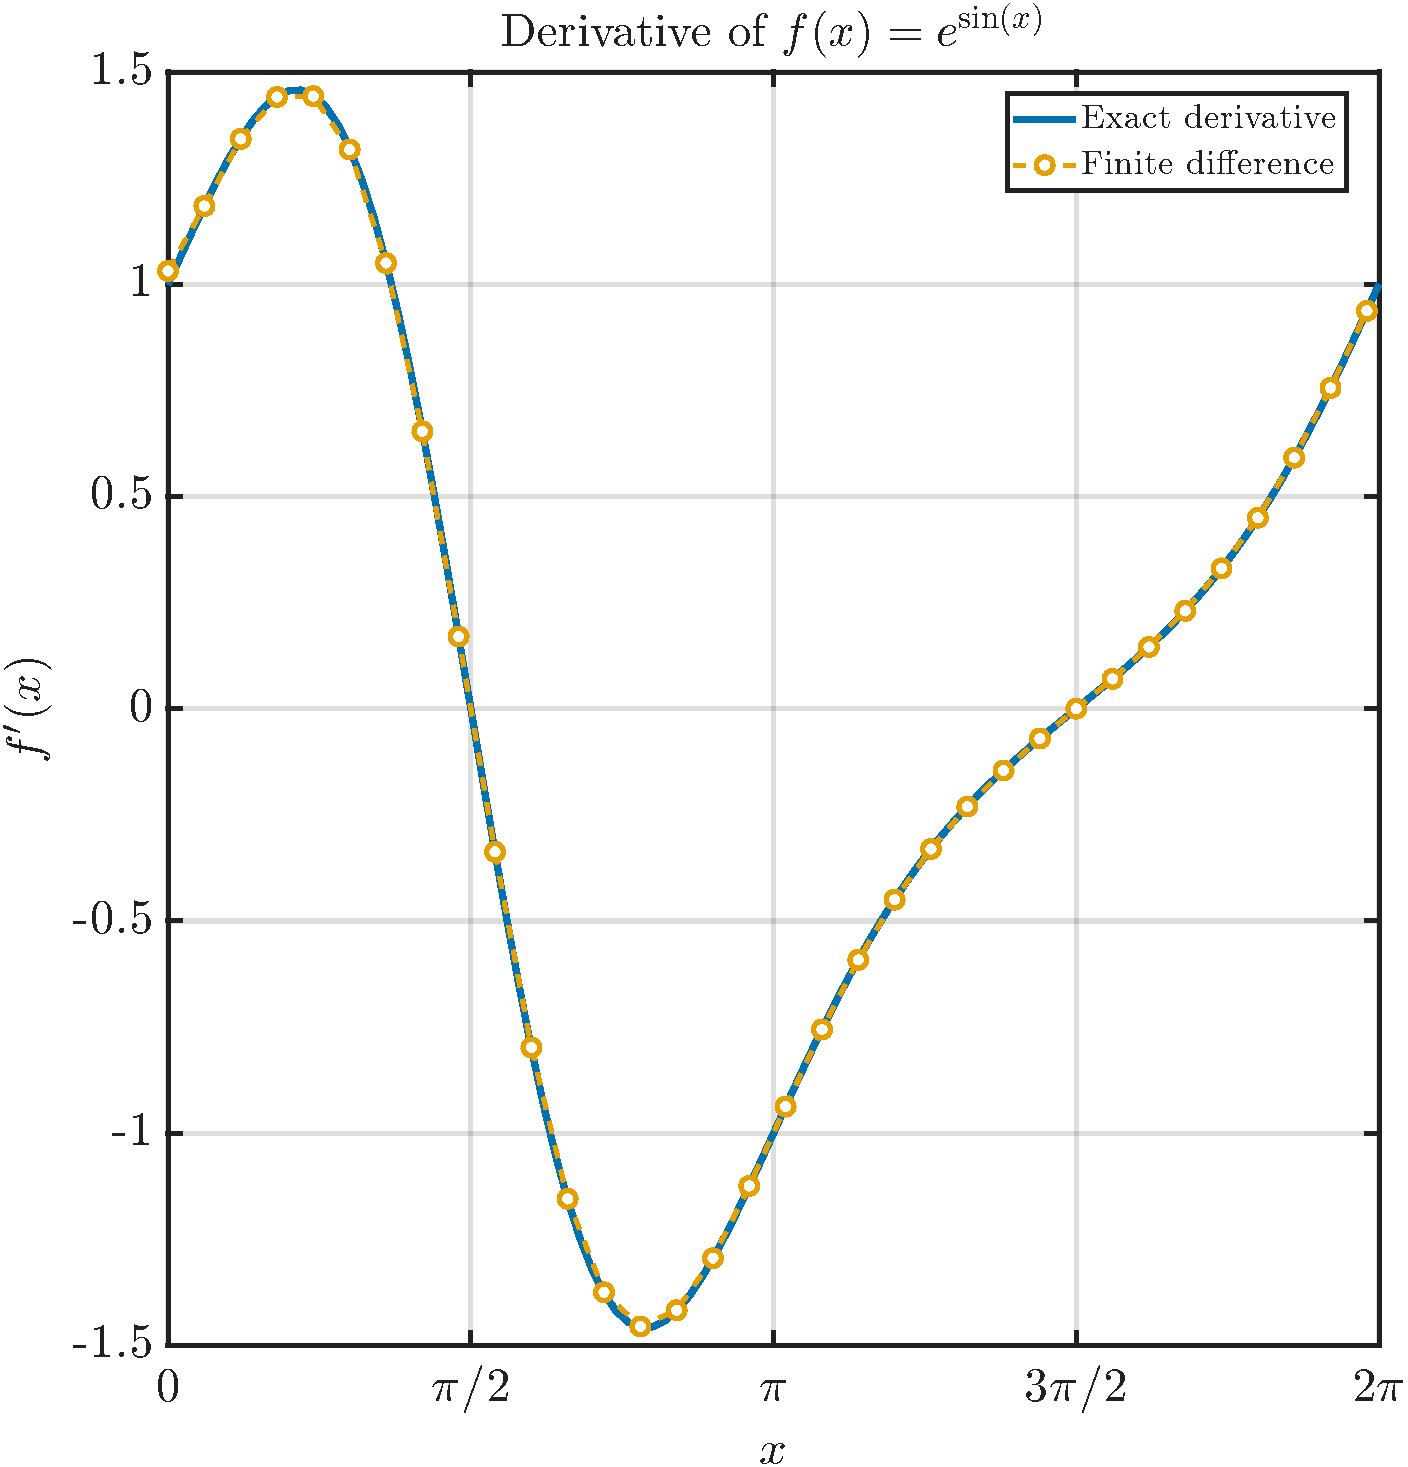
\includegraphics[width=0.80\textwidth, height = 0.55\textheight]{finiteDifferenceQ1a.pdf}
    \caption{Comparison of the exact derivative of
    $f(x)=e^{\sin x}$ with the finite difference approximation.}
    \label{fig:finite-difference}
\end{figure}


\newpage By inspection, the method of approximating the derivative of $f(x)$ by finite differences is remarkably accurate when domain is discretized into grid with $N=100$ points. To achieve this result, we used first order one-sided differences on the endpoints, left and right-sided on left and right endpoints, respectively, discretretized the grid into 100 points, and set the difference between points to $2\pi / 100$. We aim to more rigorously characterize the error in the next part.


    \item Show a relative error convergence plot by plotting the relative error on the y-axis and the grid size $N$ on the x-axis. Measure relative error as
    $$Err = \frac{\Vert f'(x) - f'_n(x) \Vert_p}{\Vert f'(x) \Vert_p}.$$
    \noindent Plot the error using both the $p=\infty,2$ norms in a log-log scale. The relative errors should be lines with slopes 1 and 3/2 respectively, i.e. it scales with $\displaystyle \frac{1}{N}, \frac{1}{N^{3/2}}$. Extra Credit: The $3/2$ slope is strange, why is that happening?

\begin{figure}[H]
    \centering
    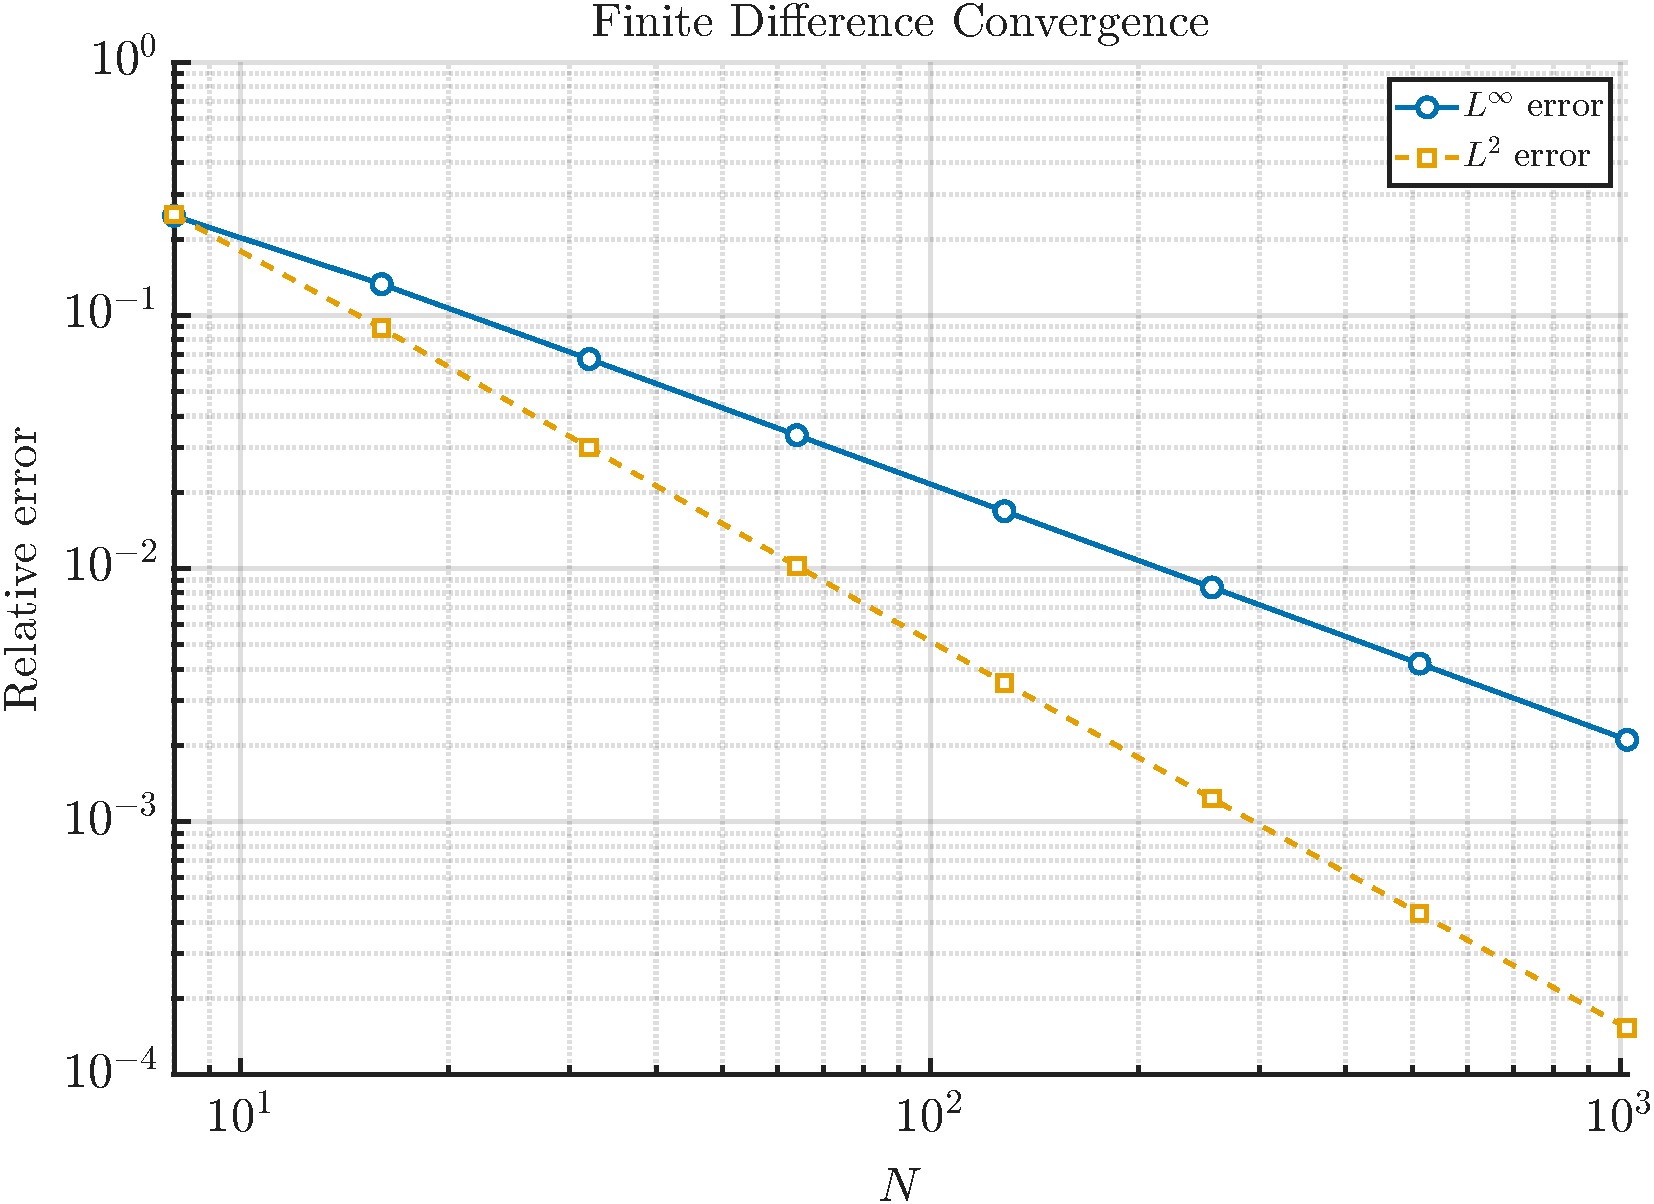
\includegraphics[width=0.80\textwidth, height = 0.55\textheight]{convergenceq1.pdf}
    \caption{$L^{\infty}$ and $L^{2}$ error log-log plot}
    \label{fig:finite-difference}
\end{figure}

As expected, the error decreases with increasing N. In particular, $Err$ scales with $1/N$ with $L^{\infty}$ norm and $1/N^{3/2}$ with the standard euclidean norm. The $L^{\infty}$ norm is equivalent to taking the maximum of the components, so it makes sense that the error scales with $1/N$, as the largest component in this case is the largest error, i.e, the first order error found at the endpoints. Interestingly, we should expect the $L^{2}$ norm to grant an error that scales with $1/N^{2}$, since $f_{n}$ is a second order approximation. However, it is trivial to show that the error's numerator term is dominated by the endpoints:
\begin{align*}
  O(\lVert f'(x)\rVert_{2}) = \sqrt{\sum O(1)^{2}} = O(\sqrt{N}) \\
  O(\lVert f'(x)-f_{n}'(x)\rVert_{2}) = \sqrt{2O(1/N)^{2}+\sum O(1/N^{2})^{2}} = O(1/N)
\end{align*}
from which we can write $O(Err) = O(1/N^{\frac{3}{2}})$. Hence, the first order approximation at the endpoints ultimately determines how the error scales with grid size.
\end{enumerate}

\vspace{0.5cm}

\noindent \textbf{Problem 2: Second-order derivatives}
Repeat problem 1 but compute the second derivative $f''(x)$. Assume periodicity and wrap around the grid instead of using one-sided finite differences. \\

For this problem we find the second derivative of the function analytically:
\[
  f''(x) = e^{\sin x}(\cos^{2}x-\sin x)
\]

and we use the second order centered approximation:
\[
  f''(x_i) \sim \frac{f_{i+1}-2f_{i}+f_{i-1}}{\Delta x^{2}}
\]

We discretize the grid into 100 points, and take advantage of the periodicity of $f$ to avoid relying on first order one-sided differences at the end points. We utilize the circshift function in matlab to realize this.

\begin{figure}[H]
    \centering
    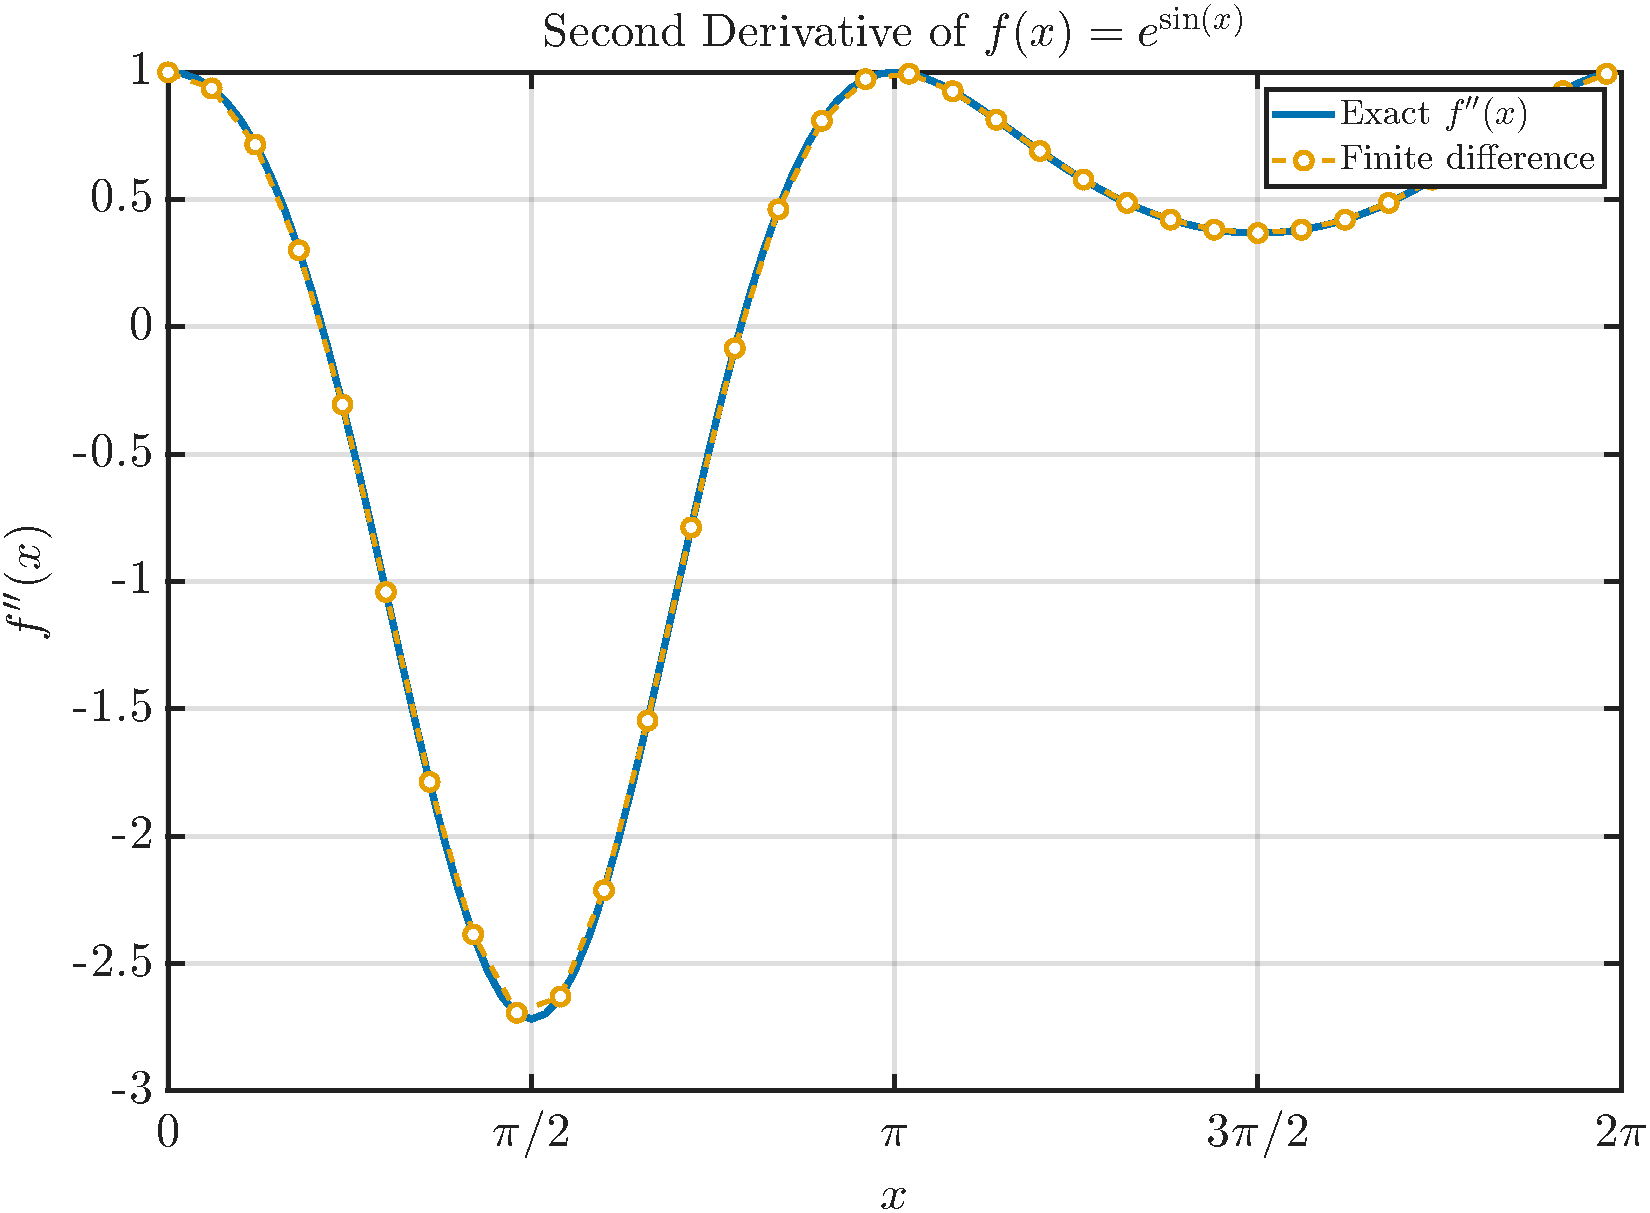
\includegraphics[width=0.80\textwidth, height = 0.55\textheight]{secondDerivative.pdf}
    \caption{Comparison of the exact second derivative of
    $f(x)=e^{\sin x}$ with the finite difference approximation.}
    \label{fig:finite-difference}
\end{figure}

In this case, we see that the second ordered centered difference method does a good job of approximating the second derivative of $f$, and we proceed to graph the error under the $L^{2}$ and $L^{\infty}$ norms. Since we are not using first order approximations anywhere, we expect to not see drastic differences in the slopes of the errors in log log plot as in the previous question.
\begin{figure}[H]
    \centering
    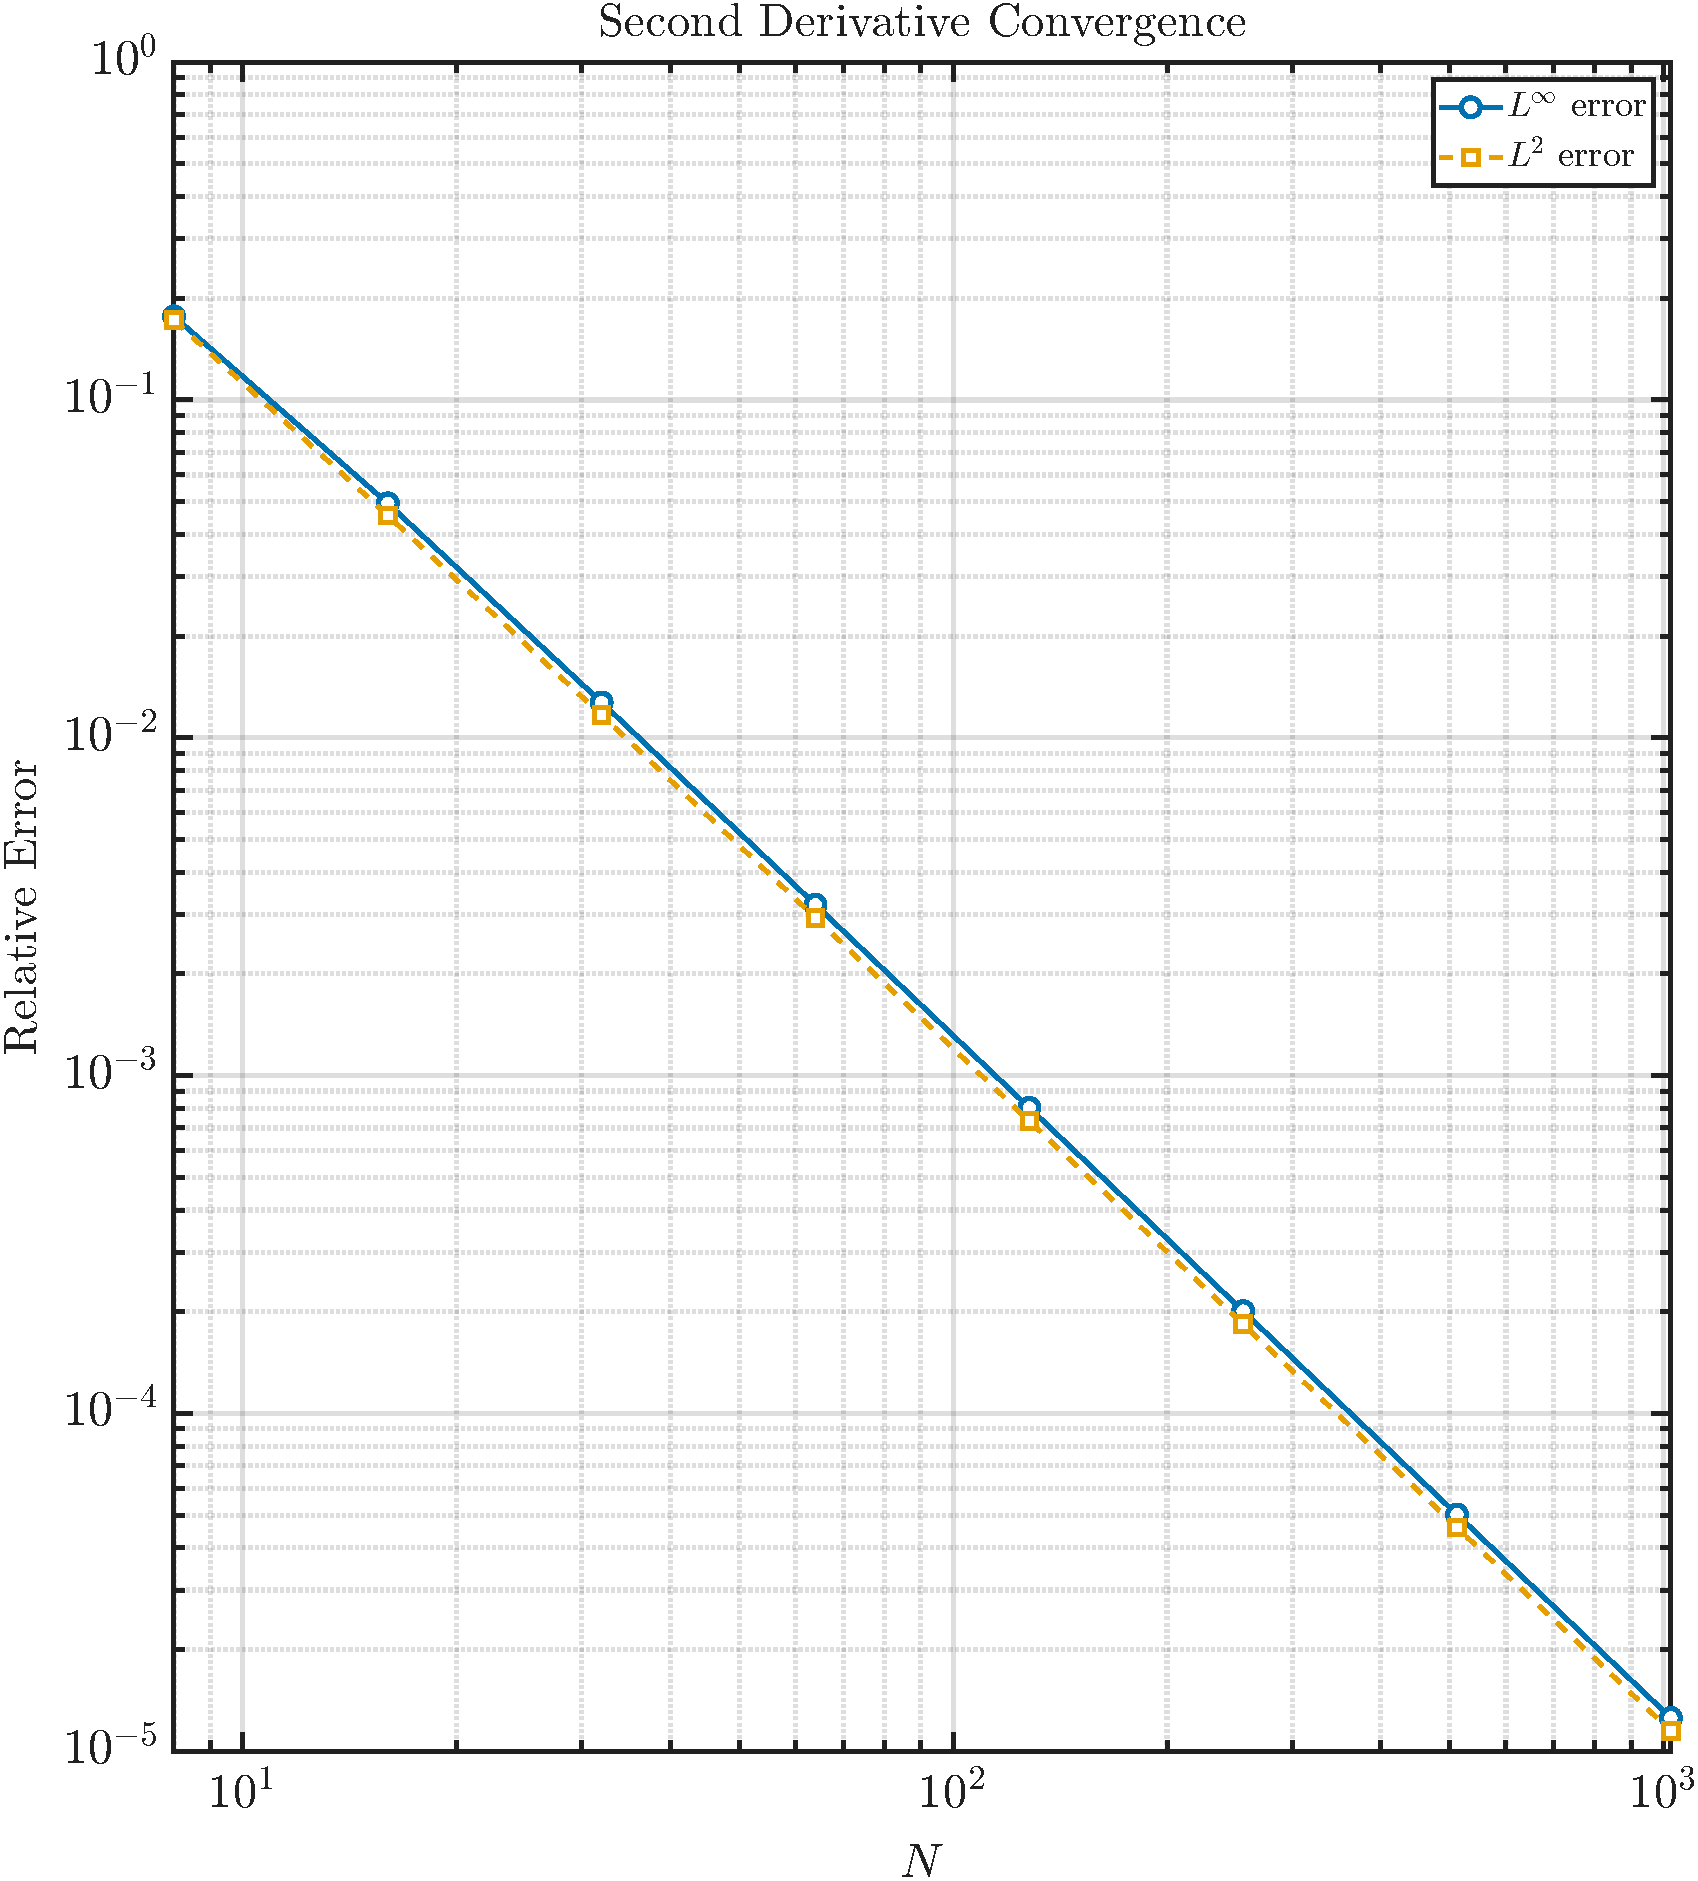
\includegraphics[width=0.80\textwidth, height = 0.55\textheight]{secondDerivativeConvergence.pdf}
    \caption{$L^{2}$ and $L^{\infty}$ error log-log plots for approximate soluton of second derivative}
    \label{fig:finite-difference}
\end{figure}

As expected, the two lines are effectively parallel. In particular, line has slope $-2$, and so the error scales with $1/N^{2}$. Since we do not have any first order approximations, the maximum of the errors for each N is not dominated by the first order approximations, and neither is the numerator of the $L^{2}$ norm. Hence, we have what we expect, error of order $\Delta x^{2}$, or of the order $1/N^{2}$
\vspace{0.5cm}

\noindent \textbf{Problem 3: ODE}
Consider the ODE
$$\dv[2]{u}{x} + \sin(x) \dv{u}{x} + u(x) = f(x)$$
defined on $0 \leq x \leq 5$. Solve the ODE using second-order finite difference methods with the Dirichlet conditions. Use $u(x) = \sin(x)$ to test your solution by finding boundary conditions and the necessary forcing function $f(x)$. Show an error plot that proves your method converges with second order.

We use centered second order differences to approximate $u''$ and $u'$, after discretizing the domain so that $h = 5/N$, $x_{i} = ih$ for $i = 0,\dots, N$, and letting $U_{i} \sim u_{x_{i}}$:
\[
  u''(x_{i}) \sim \frac{U_{i+1}-2U_{i}+U_{i-1}}{h^{2}}
\]

and

\[
  u'(x_{i})\sim \frac{U_{i+1}-U_{i-1}}{2h}
\]
Substituting into the ODE:

\begin{align*}
  \frac{U_{i+1}-2U_{i}+U_{i-1}}{h^{2}}+\sin x_{i}\frac{U_{i+1}-U_{i-1}}{2h}+U_{i} = f(x_{i}) \\
  (\frac{1}{h^{2}}-\frac{sin x_{i}}{2h})U_{i-1}+(1-\frac{2}{h^{2}})U_{i}+(\frac{1}{h^{2}}+\frac{sin x_{i}}{2h})U_{i+1} = f(x_{i})
\end{align*}
Letting $a_{i}.b_{i},c_{i}$ be the coefficients for $U_{i-1},U_{i},U_{i+1}$, respectively, implies the following relation:
\[
  a_{i}U_{i-1}+b_{i}U_{i}+c_{i}U_{i+1} = f(x_{i})
\]
for $i = 1, \dots N-1$, which implies the following system:
\[
\begin{bmatrix}
b_1 & c_1 & 0 & \cdots & 0 \\
a_2 & b_2 & c_2 & \ddots & \vdots \\
0 & a_3 & b_3 & \ddots & 0 \\
\vdots & \ddots & \ddots & \ddots & c_{N-2} \\
0 & \cdots & 0 & a_{N-1} & b_{N-1}
\end{bmatrix}
\begin{bmatrix}
U_1 \\
U_2 \\
U_3 \\
\vdots \\
U_{N-1}
\end{bmatrix}
=
\begin{bmatrix}
f_1 - a_{1}u(0) \\
f_2 \\
f_3 \\
\vdots \\
f_{N-1} - c_{N-1}u(5)
\end{bmatrix}.
\]

The solution to this system gives us an approximate solution to the ODE with second order error.

We now impose the dirichlet conditions. Assuming, $u(x)=\sin x$ and substituting into the ODE,
\[
  -\sin x +\sin x\cos x +\sin x =f(x)
\]

which implies $f(x) = \sin x \cos x$. We also have $U(0) = \sin 0 = 0$, and $U(5) = \sin 5$. So we get:

\[
\begin{bmatrix}
b_1 & c_1 & 0 & \cdots & 0 \\
a_2 & b_2 & c_2 & \ddots & \vdots \\
0 & a_3 & b_3 & \ddots & 0 \\
\vdots & \ddots & \ddots & \ddots & c_{N-2} \\
0 & \cdots & 0 & a_{N-1} & b_{N-1}
\end{bmatrix}
\begin{bmatrix}
U_1 \\
U_2 \\
U_3 \\
\vdots \\
U_{N-1}
\end{bmatrix}
=
\begin{bmatrix}
\sin x_{1}\cos x_{1} \\
\sin x_{2}\cos x_{2} \\
\sin x_{3}\cos x_{3} \\
\vdots \\
\sin x_{N-1}\cos x_{{N-1}} - c_{N-1}\sin 5
\end{bmatrix}.
\]
Solving the system numerically, we plot the $L^{\infty}$ error:

\begin{figure}[H]
    \centering
    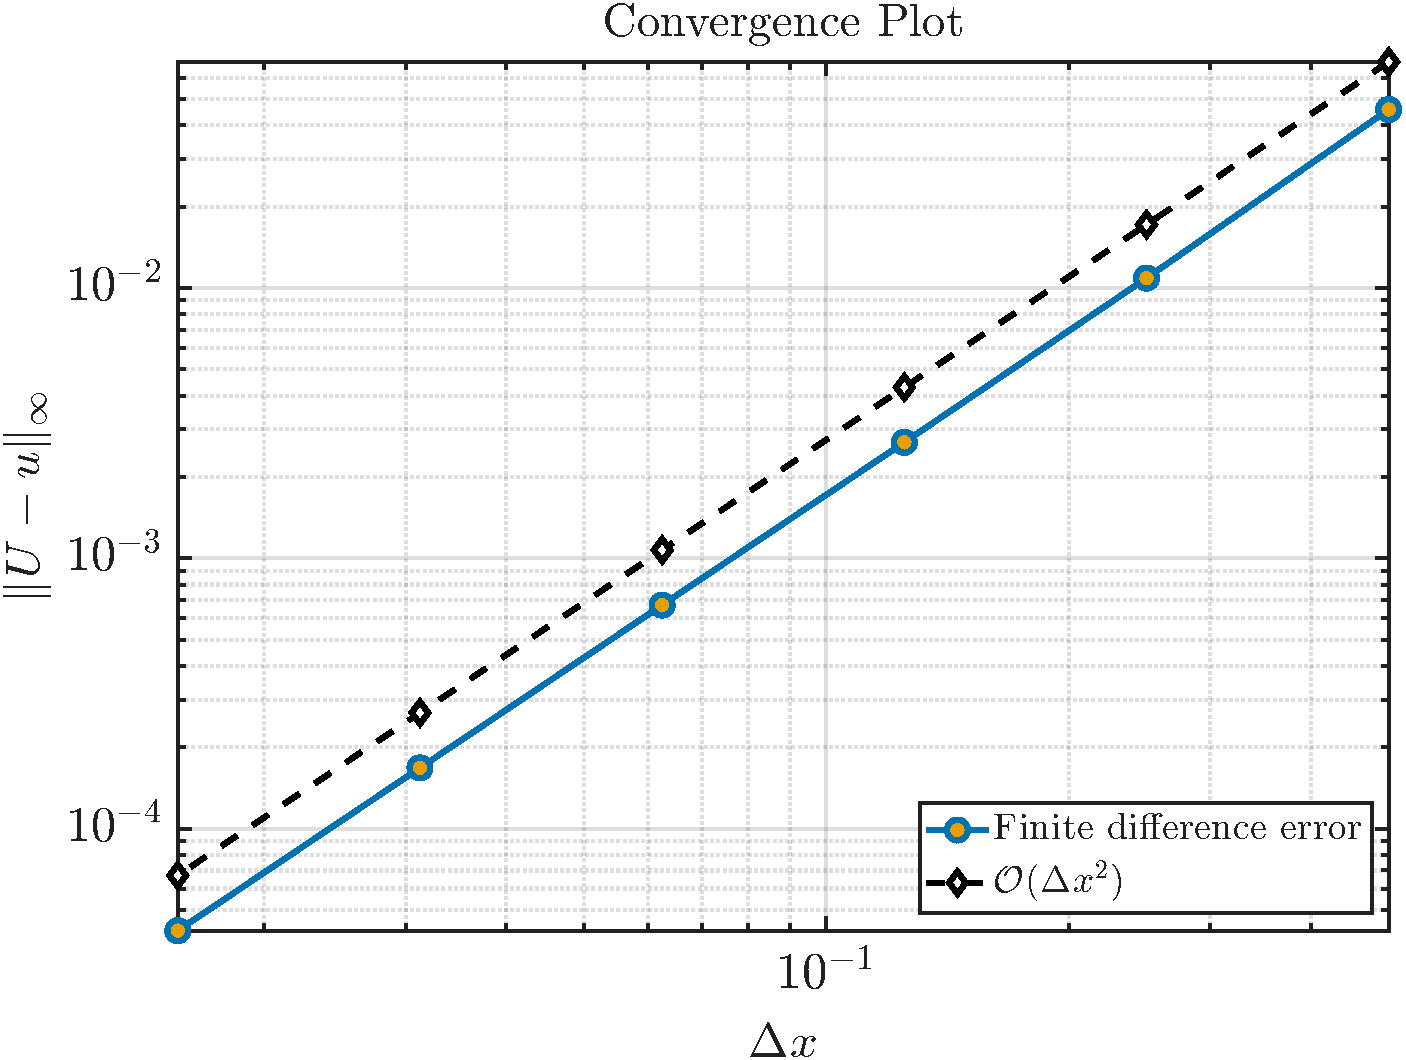
\includegraphics[width=0.80\textwidth, height = 0.55\textheight]{convergencePlot.pdf}
    \caption{Finite difference error plotted alongside $O(\Delta x^{2}$) with log-log scale}
    \label{fig:finite-difference}
\end{figure}
After computing the $L^{\infty}$ error of our approximate solution to the ODE, we see that as $N$ grows large, $\Delta x$ approaches 0, and the error scales with $1/N^{2}$, or $\Delta x^{2}$. It is parallel to a line of order $\Delta ^{2}$. This proves the method converges with second order.

\vspace{0.5cm}
\noindent \textbf{Problem 4: Poisson Equation}
Use finite difference methods to solve the Poisson equation $\nabla^2 u = f(x,y)$ in the domain $x \in [0, 5], y \in [0, 5]$. Use the test solution $u(x,y) = \sin(x)\cos(y)$.

\begin{enumerate}
    \item Apply Dirichlet conditions on all boundaries so that $u(x,y)$ satisfies the PDE and the boundary conditions, and show a plot of your solution and a second order convergence plot (similar to the first three problems).
    \item Modify your code to apply Neumann conditions on all boundaries. \textbf{This won't work.} Why not? -- both in terms of the linear algebra and in terms of the actual PDE we want to solve. Suggest a solution to the issue.
\end{enumerate}

\vspace{0.5cm}
\noindent \textbf{AI Statement}
An LLM (ChatGPT 5.6) was prompted with the textbook on the numberFactory github and the matlab code for each assignment to generate all plot code in the convention required (i.e to implement accessbiliity features). Further,an Opencode agent using GLM 5.3 Flash was used to generate the README.md. The matlab code and latex document outside of plots was not generated using LLM.

\end{document}
